\documentclass[../main.tex]{subfiles}
\graphicspath{{\subfix{../}}}
\begin{document}

\chapter{A New Way of Working using Information Models}
\label{ch:Chapter 3}




\section{Problem Statement}
\label{ch:Section 1.1}
Facility assets in the energy industry are becoming increasingly complex.
There is a need for better communication between organisations, people, and IT systems. Actors in the industry use
different methods, tools, and work processes to develop a facility asset. This misalignment is seen:

\begin{itemize}
  \item Along with the Capital Value Process (CVP);
  \item Along the supply chain; and
  \item Between disciplines and systems within the same facility asset.
\end{itemize}
The consequences of this are loss of information, risk of safety and quality breaches, duplication of work,
a lot of manual mapping, reduced possibilities for re-use of concepts and design, lock-in to a portfolio of
applications, and a lot of company-specific requirements that are tuned to fulfil needs for a certain portfolio of
applications.

\autoref{fig:Figure 1} illustrates the problem of today's way of working. The figure shows the \emph{logical} flow of value
creation during an industrial investment and development project, the actual execution schedule will have
many overlaps and iterations that are intentionally left out.

\begin{figure}[h]
  \centering
  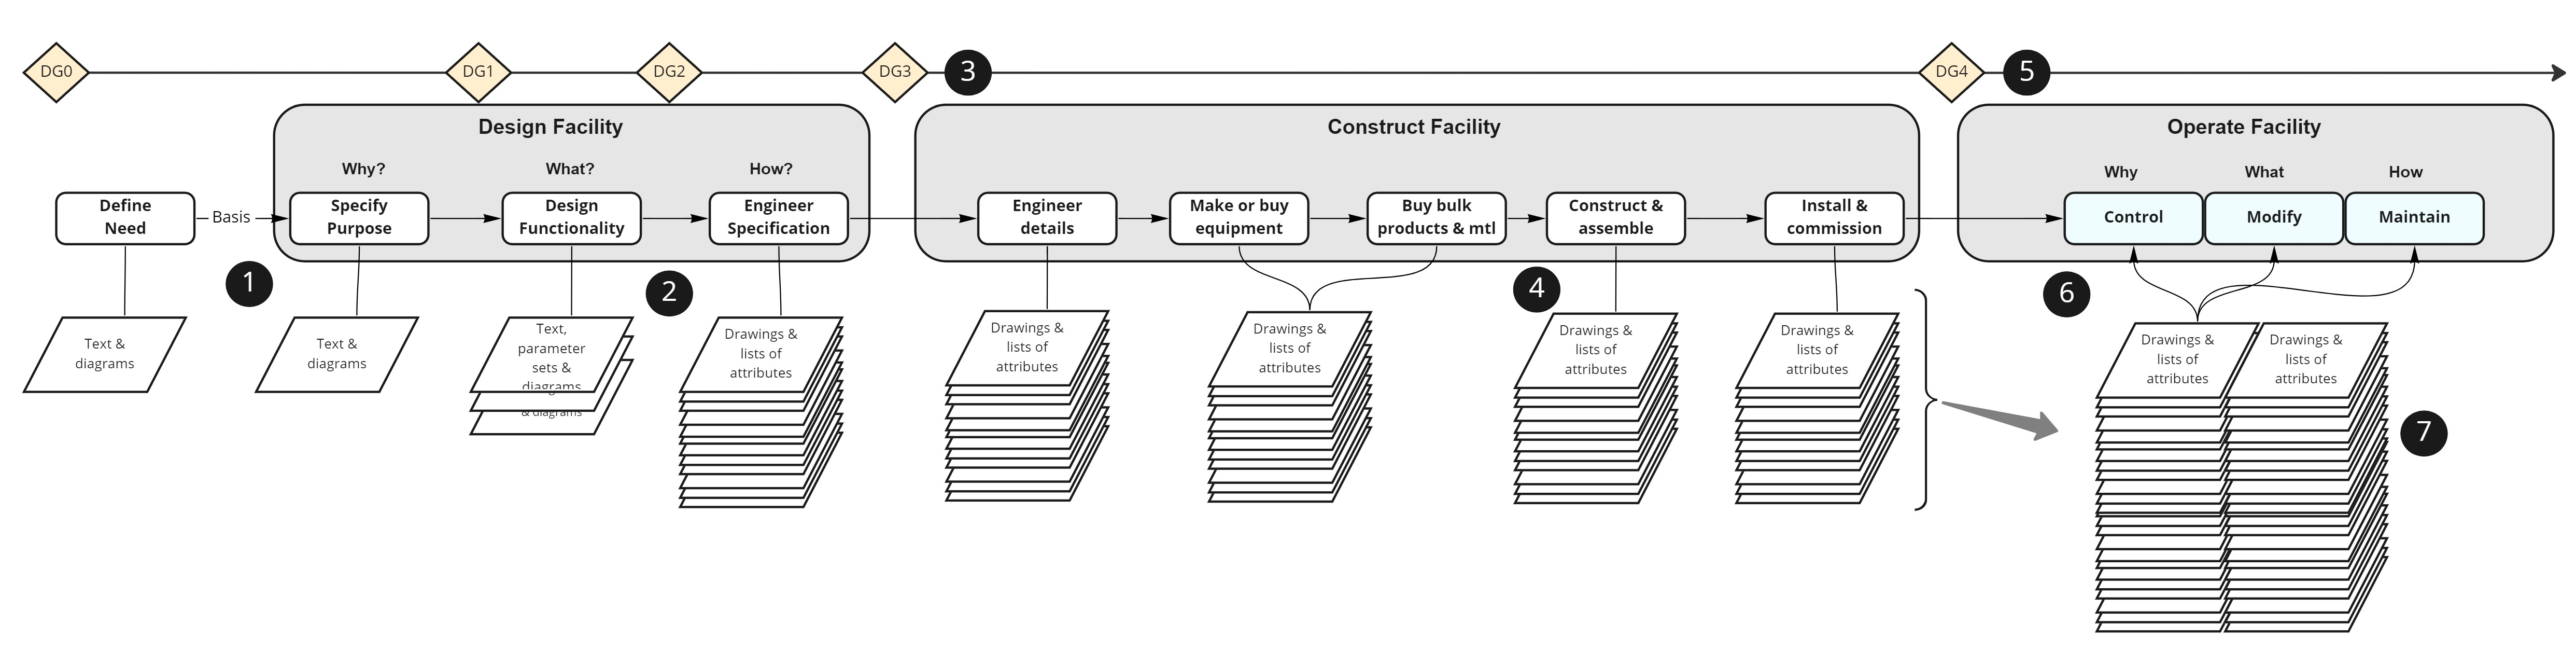
\includegraphics[width=1\textwidth]{img/IMFmanual-img001.jpg}
  \caption{Current documentation practice during an industrial
    investment and development project.}
  \label{fig:Figure 1}
\end{figure}


When a facility asset is developed today, the work begins by defining the overall requirements and functionality
(DG0). The result is typically contained in a few documents, which means that at this stage a holistic description is
feasible~\ding{182}. As the work progresses into the design phase of the facility asset, more specialised discipline
expertise is necessary (DG1 and DG2). Since the way of working is document-based, the result is an increasing number
of documents. This leads to a fragmentation of information spread across documents, due to the inherent features of
their format. Because of this fragmentation, it becomes increasingly difficult to maintain a holistic description of the
facility asset. The result is extensive interface coordination between discipline experts~\ding{183}.

When the investment decision is made to execute the construction of the facility asset (DG3)~\ding{184}, the number of
documents produced grows exponentially as the supply chain involving both contractors, suppliers, and manufacturers
ramp up their deliveries for construction, installation, and commissioning of the facility asset~\ding{185}. At this
stage, and likely to have started earlier in the CVP, a lot of information in documents is duplicated, resulting in
several sources of the same information. The consequence of this is labour-intensive work to
    prevent quality deviations and HSE incidents.

When the operation (DG4) and handover to the operator takes place~\ding{186}, information is fragmented and lacks
relational information. This often results in a need to ``re-engineer'' the solution to establish the holistic view
necessary to maintain, control and evolve the facility asset~\ding{187}.

It is worth noting that reduced information quality can reduce the decision quality and is often costly and
inefficient to manage.

\section{Requirements to  Solution}
\label{ch:Section 1.2}
The objective of the Information Modelling Framework (IMF) is to enable
a transition from the current documentation practice discussed in \autoref{ch:Section 1.1}, to the use of information
  models as a way of capturing and expressing information about facility assets.

To achieve this transition, the solution  must facilitate for:

\begin{itemize}
  \item Incremental implementation. Thus, handle both a new information model practice and the transition towards it,
        yet not require existing applications and tools to be replaced.
  \item Scalability across disciplines, work processes, and the value chain. The method needs to be granular enough to
        support any level of complexity and detail, depending on the need and where in the process the SMEs are.
  \item Ease of use. Be made intuitive to the extent that the SMEs themselves are users of the framework. Thus, the
        method must support and allow existing discipline design workflows.
  \item Utilisation and promotion of shared libraries and existing standards.
  \item Open protocols for exchange of facility asset information and provide a format which enables automated
        verification and augmented engineering extensions.
\end{itemize}

\section{Using Information Models}
\label{sec:userinformationmodel}
To solve the problems discussed in \autoref{ch:Section 1.1}, fundamental
changes in the way we capture and represent information are needed. Used properly, information models in
combination with reference data libraries (RDLs) include the features necessary to handle the problems of the current
document practice.

\autoref{fig:Figure 10} illustrates a new way of working using information models through the logical flow of value
creation during an industrial investment and development project. The actual execution schedule will have many
overlaps and iterations that are intentionally left out.

\begin{figure}[htb]
  \centering
  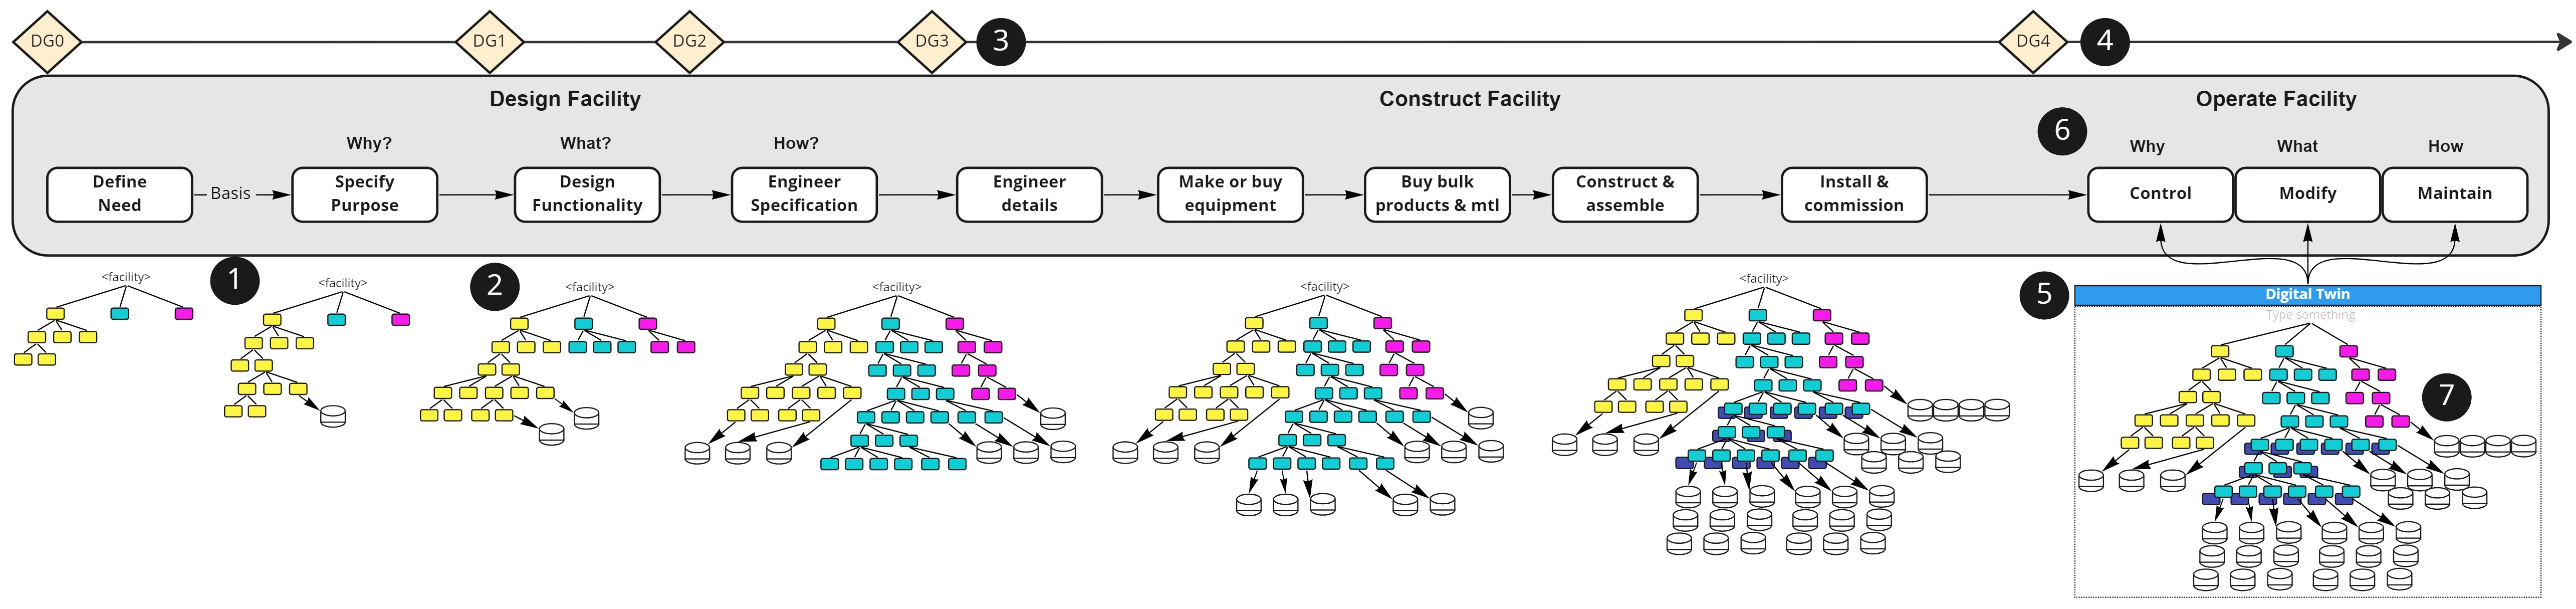
\includegraphics[width=1\textwidth]{img/IMFmanual-img010.jpg}
  \caption{Using information models instead of documents during an
    industrial investment and development project.}
  \label{fig:Figure 10}
\end{figure}

The overall requirements to functionality of the facility asset (DG0) are captured in an information model~\ding{182}.
As the work progresses into the design phase of the facility asset, several more detailed information models are
created by discipline expertise to mature the design (DG1 and DG2)~\ding{183}. Due to the inherent features of the
(machine-readable) format, the information models can be continuously checked for design flaws by an automated work process. Furthermore, the fragments of information, now represented through several
information models, can be integrated along the way to ensure a consistent design and a valid description of the
facility asset on a holistic level.

When the investment decision is made to execute the construction of the facility asset (DG3)~\ding{184}, information
models describing parts of the facility asset are produced in large quantities by the supply chain.

When approaching operation (DG4) and handover to operator takes place~\ding{185}, the resulting information model, can
be thought of as a \emph{model-of-models}, containing the historical context and all design decisions made all the way back to DG0~\ding{186}.
The holistic description and the contents of the facility asset is available at any granular level as required to operate, control, maintain, and later do modifications on the facility asset~\ding{187}. Furthermore, access to
information is not restricted by documents and formatting but can be navigated freely~\ding{188} and maintained efficiently.

\section{New Methods, Roles, and Competencies}
\label{sec:newmethodsroles}
The new way of working implies new roles and requires new
competencies. The following roles are relevant:

\begin{itemize}
  \item The \emph{subject matter expert} (SME). SMEs are experts on discipline engineering. For example, a process
        engineer who develops the design of the main processing system, or an electrical engineer who develops the design of
        the electrical supply and distribution.
  \item The \emph{system engineer} is an expert on system integration. For example, a system engineer is responsible
        for coherent integration of system designs from, e.g., different disciplines, different phases of the project
        lifecycle and different parties in the value chain.
  \item The \emph{data engineer} is an expert on the flow of data between IT systems and applications. For example, a
        data engineer manages the export of data from a model authoring application into an engineering register system.
  \item The \emph{knowledge engineer} is an expert on knowledge representation and semantic technology. For example, a knowledge engineer manages
        the validation and integrity verification of the model of a design.
\end{itemize}

\begin{figure}[htb]
  \centering
  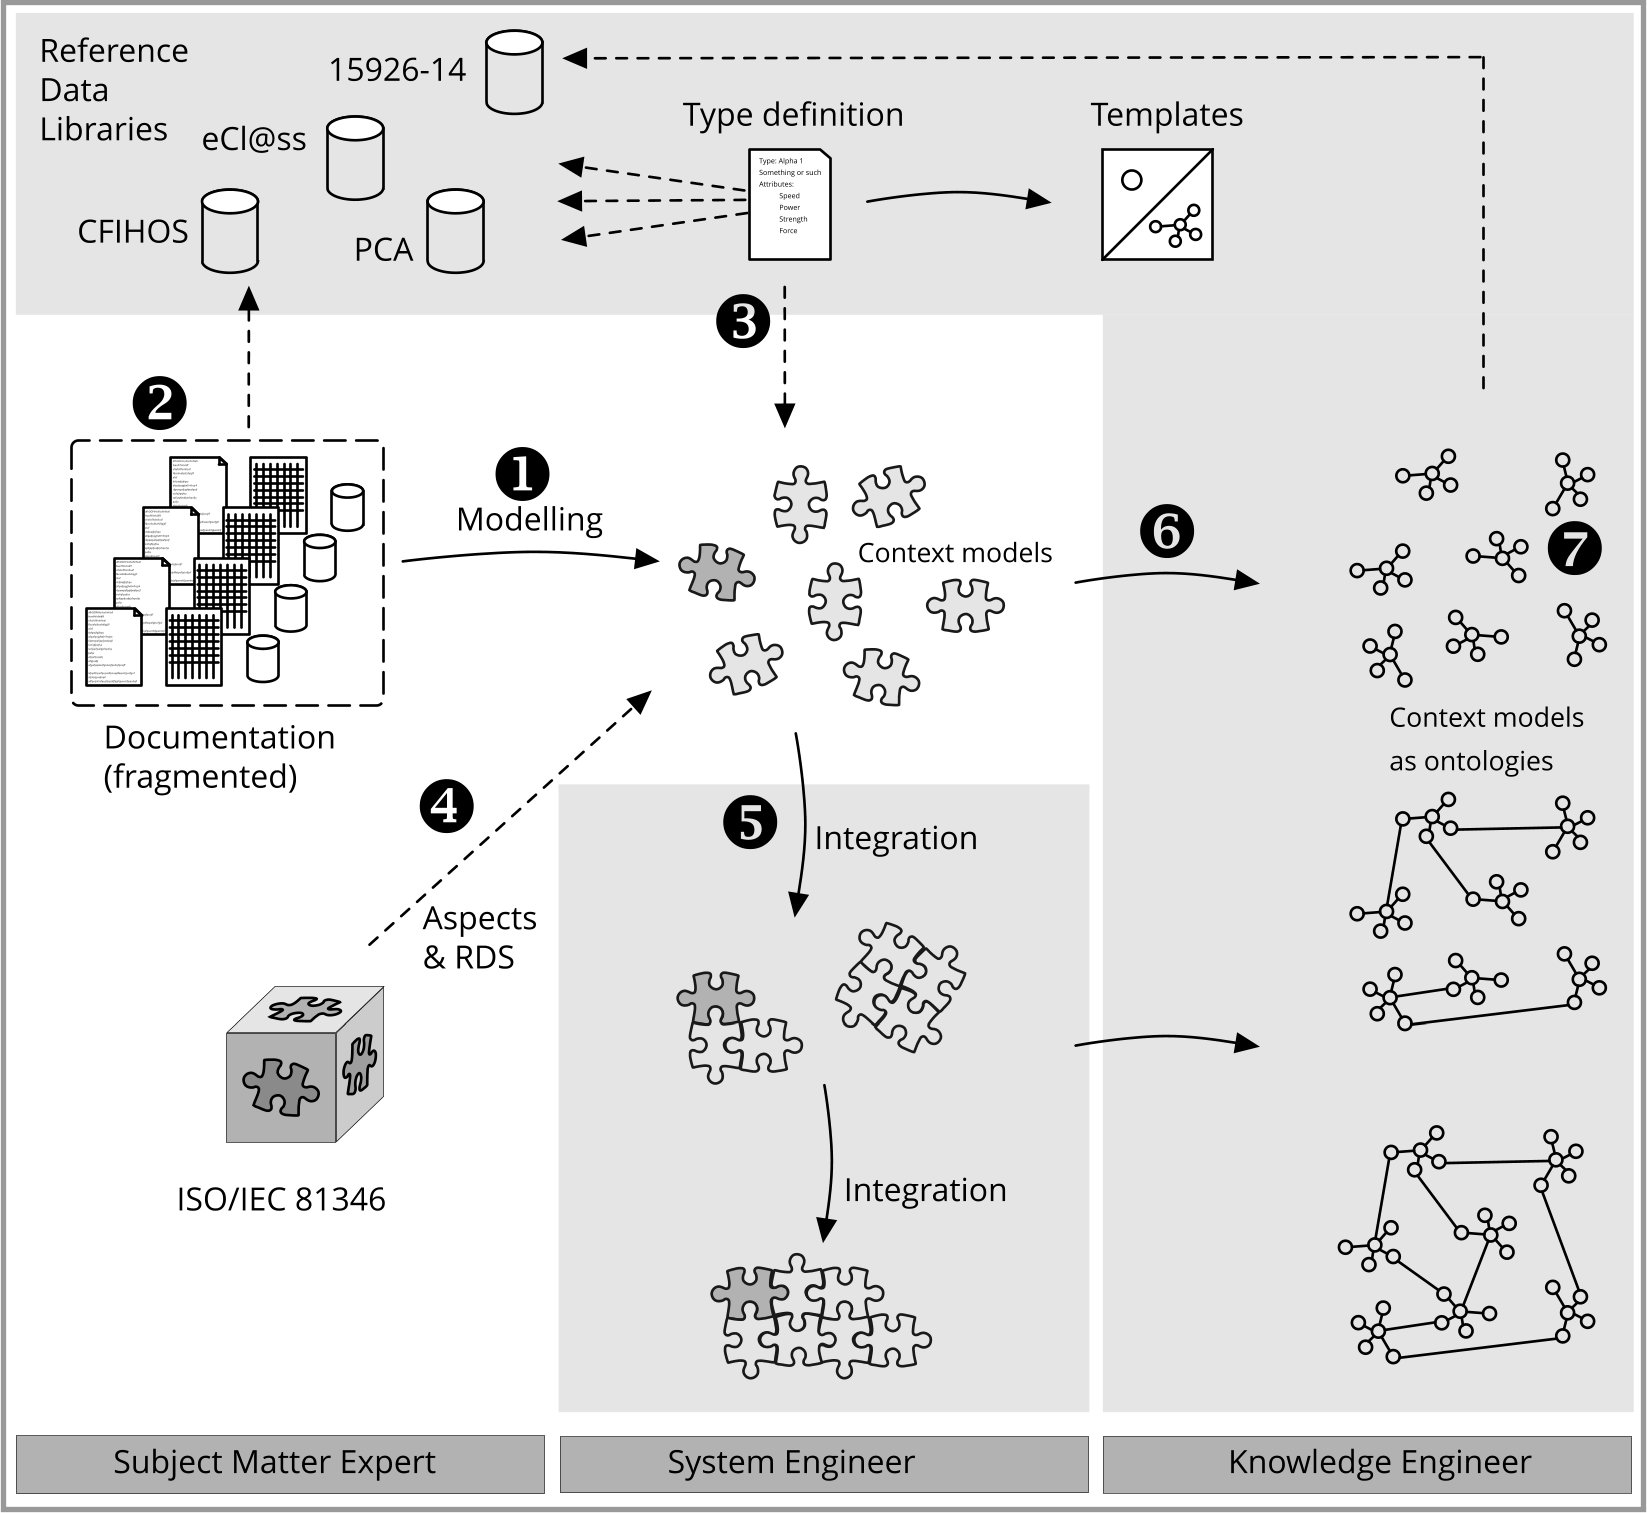
\includegraphics[width=1\textwidth]{img/IMFmanual-img011.jpg}
  \caption{Different expertise and how they enable information modelling of facility assets.}
  \label{fig:Figure 11}
\end{figure}

Engineering and design is a process of making a series of decisions founded on subject matter expertise and governed
by requirements and limitations. This is the domain of SMEs and system engineers, but the new way of working allows a
significant shift in focus away from \emph{formatting} of information, and towards \emph{creating} information.
It is less constrained by document formats and instead allows a much more flexible and incremental way of creating a
design. This will have an impact on how the work is optimally allocated into different roles.

The SME role is by definition to hold expertise on a defined subject, usually a single discipline, but the new way of
working will reward an approach of also working across disciplines that are interlinked and interdependent, thus
reducing time-consuming coordination effort. As systems thinking is a fundamental part, the system engineer role may
have a stronger impact, in particular when integrating segments of models into a whole, and when managing how systems
interact.

While the data engineer has conventionally had more focus on batch transfer of data between systems, this role will
need to strengthen the focus on publishing and sharing of model data, and on leveraging semantic technologies. A
significant value of modelling is that it allows use of advanced semantic technologies and mechanisms for
machine-based validation and verification. The role of the knowledge engineer is instrumental for achieving this.

\autoref{fig:Figure 11} illustrates how the different roles work together to enable modelling of parts of the facility asset that
then are integrated into a complete model where semantic technology is utilised to verify and validate the integrity
of the model.


SMEs model information that today is available only in fragments, commonly recorded in documents~\ding{182}.  The documents
may refer to standards, possibly exploiting reference data, such as names of shared properties and classes, and
initiatives to digitally enrich documentation format such as DEXPI\footnote{\url{https://dexpi.org/specifications/}}
\ding{183}.  When modelling, the SME creates the building blocks of the model from definitions held in a common
industry library, a reference data library~\ding{184}, enabling the re-use of well-proven design patterns (e.g., type
of pump configuration). The building blocks are put together into a model in accordance with the rules and
structures of IMF that build on the IEC/ISO81346 O\&G standard~\cite{81346-OG}~\ding{185}.

IMF does not require modelling to be done in one single model, something which often is implied when referring to data-centric
or model-centric ways of working. Instead, the modelling can be distributed across many smaller IMF models, here shown as puzzle
pieces, that the system engineer later can bring together as a complete puzzle~\ding{186}. IMF models can be
translated~\ding{187} into semantically enriched models that enable the knowledge engineers to exploit verification techniques such as automated
reasoning~\ding{188}.

%
\section{The IMF Ecosystem}
\label{ch:Chapter 7}

- icons
- best practices, recommendations
- end-to-end example?

In order to describe a typical set up of an IMF Ecosystem, we use the
following terminology:

\begin{description}
\item[{IT Ecosystem}] IT ecosystem refers to an orchestrated
  collection of components: IT systems, tools, actors and roles, and
  how they interact to achieve a specific goal.

\item[{Data}] Data refers to the information that is stored,
  processed, and transmitted within the IT ecosystem. It can include
  text, numbers, images, audio, video, or any other form of digital
  content.

\item[{Language and Format}] Language and format refer to the methods
  and standards used for communication and data representation within
  the IT ecosystem. This includes data exchange protocols and data
  formats that dictate how data is structured and transmitted.

\item[{IT Systems}] IT systems are the major components within the IT
  ecosystem that store data and provide services that process data.
  Typical examples are databases and server-side applications.

\item[{Tools}] Tools refer to software applications, utilities, or
  programs that are used to perform specific tasks or functions,
  typically on data, within an IT ecosystem. They can be used for data
  analysis, editing, monitoring, or other purposes. Typical examples
  are client side desktop applications.

\item[{Service}] A service is a specific functionality or capability
  offered by an IT system or tool. It defines what the IT system or
  tool can do and how it can be accessed or utilized by
  actors. Typical examples of services are data validation, identifier
  management, and user authentication.

\item[{Actors}] Actors represent entities or users that interact with
  IT systems and tools. They can be individuals, external systems, or
  automated processes that initiate actions or provide input to the
  system.

\item[{Roles}] Roles represent the different functions or
  responsibilities that individuals or components within a IT
  ecosystem have. They define who or what performs specific tasks or
  operations within the system.
\end{description}

\subsection{IMF Ecosystem Components}

\subsubsection{Reference Data}
\label{sec:reference-data}

Reference data refers to a specific type of data that provides context
or categorization for other data. It is typically static and does not
change frequently, serving as a point of reference or standard against
which other data can be compared, classified and integrated. Reference
data is used for validation, to ensure consistency and complience,
accuracy, to organise data within an IT ecosystem, and to standardise
access and use of data in the IT ecosystem.

In the IMF ecosystem, reference data appear in the form of reference
data items (classes, relations and individuals) typically defined in
international domain standards, such as ??? IDO, eCLass, ...? that
define industry shared resources such as equipment classes and units of
measure.

We also refer to standardised graphical symbols used for diagrams,
such as P\&ID diagrams, as reference data.

Reference data is typically made accessible by reference data
libraries.


\subsubsection{Reference Data Library}
\label{sec:refer-data-libr}

A reference data library (RDL) is an IT system whose main service is
to publish reference data so that it can be referred to by other systems, tools and
data. 
Additionally, an RDL may provide services like
data validation,
data analysis,
data enrichment,
data governance,
and
creation and curation of reference data.
These services are typically offered through APIs and are used via purpose built tools.

The IMF ecosystem contains different kinds of reference data
libraries:
industry terminology RDLs that contain industry shared terms such as equipment classes and units of measure; 
symbol RDLs that contain standardised graphical symbols;
and
IMF type libraries.

\subsubsection{IMF Type Library}

An IMF type library is a reference data library that publishes IMF types.

The benefits of an IMF type library, in addition to the generic benefits of reference data libraries, is to reduce the startup costs of using IMF as an IMF type library will provide useful IMF modelling patterns for use in the creation of IMF models.

In addition, an IMF type library may provide the following services:

\begin{itemize}
\item Submitting suggestions for new and updating existing IMF types.
\item Quality assurance (QA) process for approval of suggestions for
  new and updating existing IMF types. The QA workflow shall be
  transparent and offer relevant tools for an efficient and easy to
  use workflow.
\item Versioning scheme for the entries in the library.
\item APIs that allow for querying the library.
\item Classification schema for the IMF types.
\end{itemize}
  
An IMF type library should be community driven and allow users to submit new IMF types and update already
existing IMF types in the library. This will allow users across the industry and value chain to collaborate to create
high quality content. The approval process can be implemented as a peer-review where groups of SMEs can collaborate
to ensure that updates to the library have the necessary quality.

The API of the IMF type library shall offer support for required functionality in
the IMF type editor tools and IMF modelling tools.


\paragraph{Symbol Library}
\label{sec:symbol-library}

\paragraph{Data Hub}


\paragraph{Source databases}


\subsubsection{Tools}
\label{sec:tools}

\subsubsection{IMF Type Editor Tool}
An IMF type editor is used to create new IMF types, modify existing IMF types, and publish IMF types in a IMF type library.

An IMF type editor tool shall offer support for:

\begin{itemize}
  \item Search and browse for existing IMF types in IMF type libraries.
  \item Interaction with reference data library for finding and referencing reference data items such as attributes, classes.
  \item Creation of new IMF types using user interfaces adapted to SMEs.
  \item Updating existing IMF types in an IMF type library.
  \item A workflow for submitting new or updating existing IMF types in an IMF type library.
  \item A workflow for submitting suggestions for new reference data entries to a reference data library.
\end{itemize}
To increase the standardisation of the types created using an IMF type editor tool, reference data libraries
previously described shall be used for sourcing attributes, symbols, and classes for the creation of IMF types. There
should be a workflow that allows the SME to submit suggestions for new reference data entries to an RDL that are
identified as missing during the IMF type creation process.

An IMF modelling tool is used by SMEs to create and share IMF models.

An IMF modelling tool shall offer support for:

\begin{itemize}
\item A graphical user interface adapted to SMEs.
\item Searching and browsing for types in IMF type libraries.
\item Creation of IMF models using the complete spectrum of the IMF language.
\item Export and import IMF models to and from the IMF language.
\item Enabling plugins, e.g., that perform specific calculations and queries.
\end{itemize}
IMF modelling tools shall source the IMF types from an IMF type library. The sourced IMF types are then instantiated
in the modelling tool. Setting the values or references to values for the different attributes of the IMF types shall
be possible in the modelling tool.

An IMF modelling tool should provide a framework for adding plugins to, e.g., perform calculations and queries on the created
model.

\subsubsection{Languages and Formats}
\label{sec:languages-formats}


The IMF Ecosystem is intended to be an industry wide collaboration that allows transfer
of Information Models between the different parts of the value chain (operators, engineering contractors, suppliers).
To enable seamless transfer of information models between the different actors, potentially using different
applications, a standardised serialisation and data exchange format is needed.

The formal specification of the IMF language, which is also used as a serialisation and exchange format, is found in \autoref{ch:The IMF Language Formalized}.
The data exchange format is defined using widely accepted W3C standards. The IMF data exchange format is Resource
Description Framework (RDF), using any of its widely supported standardised serialisation formats. Several
serialisation formats for RDF exist, including JSON-LD, which is based on JSON, and RDF/XML, which is based on XML.
The data exchange format vocabulary is specified using the Web Ontology Language (OWL) and its grammar is
defined using the Shapes Constraint Language (SHACL).


\subsection{Scenarios}
\label{sec:scenarios}



\subsection{Implementations}
\label{sec:implementations}

\paragraph{Open-Source tool \emph{:Tyle}.}

The IMF type editor \emph{:Tyle} has been developed to offer adopters of IMF a web-based open-source IMF type
editor. :Tyle supports creation of IMF types using reference data from the PCA RDL.
:Tyle is developed as an open source project, where all users are
invited to contribute to the development of the tool by submitting code, bug reports or feature requests. Source
code, documentation and user tutorials can be found on
\href{https://github.com/mimir-org/typelibrary}{Github}.



\paragraph{Open-Source Tool \emph{Mímir}.}

The open-source IMF modelling tool \emph{Mímir} has been developed to offer adopters of IMF a web-based open-source
modelling tool. It supports creation of models, sourcing types from an IMF type library and compiling the models into
ontologies. All users are welcome to contribute to the development of \emph{Mímir} by submitting code, bug reports
or feature requests. Source code, documentation and tutorials can be found on
\href{https://github.com/mimir-org/mimir}{Github}.


\subsection{OLD below}

\begin{figure}[htb]
  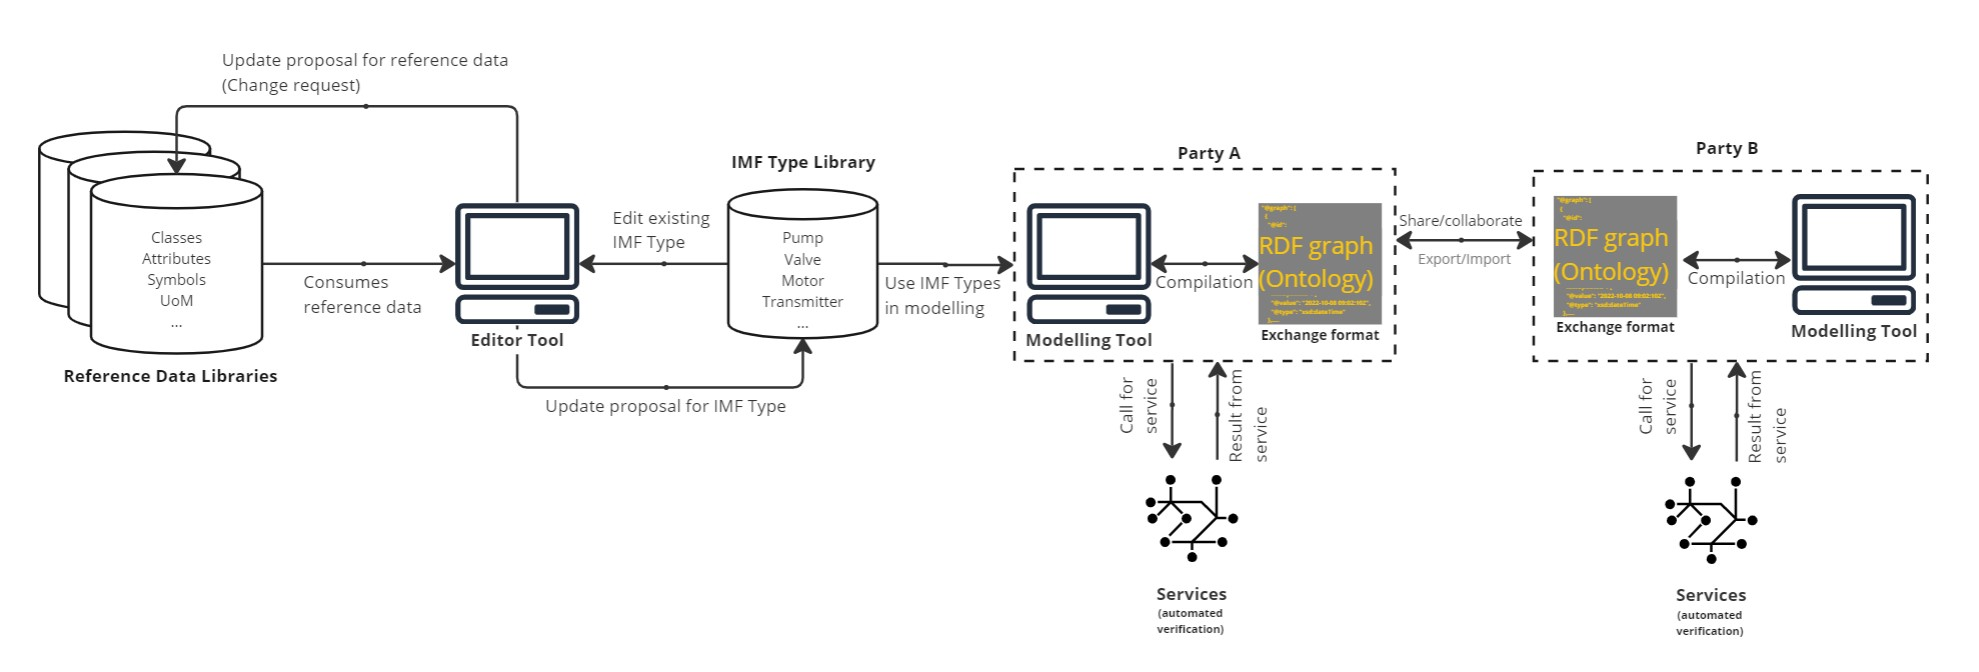
\includegraphics[width=1\textwidth]{img/IMFmanual-img072.jpg}
  \caption{Overview of the IMF ecosystem.}
  \label{fig:Figure 54}
\end{figure}


IMF will be implemented in the context of applications that serve
different parts of an ecosystem. The applications in the ecosystem should enable the engineers to create and
share information models with minimal training and independent of companies and industries. An overview of the
different components in the ecosystem is depicted in \autoref{fig:Figure 54}. The main components are reference data libraries, an IMF type library,
authoring tools, and data exchange formats. In this section all references to applications in the IMF ecosystem are
made to the type of application, not to a specific instance of the applications unless otherwise stated.


\subsection{Authoring Tools}

Authoring tools are front-end tools used by the SMEs to create IMF types and IMF
models. These tools can be implemented as standalone products or be integrated into already existing engineering
tools. 
%To offer seamless integration with the other components in the IMF ecosystem the implementation of the
Authoring tools must comply with the formal specification of the the IMF language (\autoref{ch:The IMF Language Formalized}).




%%% Local Variables:
%%% mode: latex
%%% TeX-master: "../wip"
%%% End:



\end{document}
